\subsection{Branch Unit}

\begin{figure}[H]
\centering
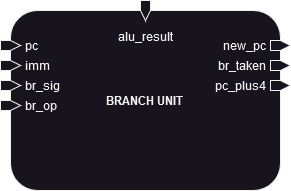
\includegraphics[width=0.5\textwidth]{../diagrams/execute/br_unit.png}
\caption{Diagram of the Branch Unit}
\label{fig:br_unit}
\end{figure}

The Branch Unit is a module that is responsible for computing the next PC. It is used in the EX stage. It uses the result of the ALU
for conditional branching to know if the branch should be taken or not.

Signals:
\begin{enumerate}[label={\textbullet}]
    \item Input: $alu\_result$, This signal is representing the result of the ALU. Used for conditional branching.
    \item Input: $pc$, This signal is representing the current PC.
    \item Input: $imm$, This signal is representing the immediate value of the instruction. It is used as an offset for the branch.
    \item Input: $branch\_sig$, This signal mark if the instruction is a branch or not.
    \item Input: $br\_op$, This signal is representing the branch operation like for example BEQ, BNE etc.
    \item Output: $new\_pc$, This signal is representing the new PC computed by the branch unit.
    \item Output: $pc\_plus\_four$, This signal is representing the PC + 4. Used to save the value of the next instruction 
    to come back at it after a branch occurred.
    \item Output: $br\_taken$, This signal is representing if the branch is taken or not. Used in the IF stage to compare 
    to the branch predictor and know if the pipeline needs to be flushed or not.
\end{enumerate}